% ============================================================================
% Pedagogical solutions - Practice 7 (Partitions & Inclusion-Exclusion).
% English, pdflatex. ASCII-clean source (no em-dash, no " -- ", no straight ").
% Compile: pdflatex twice, then view the PDF.
% ============================================================================
\documentclass[11pt,a4paper]{article}

% ---- Encoding & fonts ----
\usepackage[utf8]{inputenc}
\usepackage[T1]{fontenc}
\usepackage{lmodern}

% ---- Math ----
\usepackage{amsmath,amssymb,amsthm}
\usepackage{mathtools}

% ---- Layout ----
\usepackage[margin=2.3cm]{geometry}
\usepackage{enumitem}
\usepackage{booktabs}
\usepackage{array}
\usepackage{colortbl}

% ---- Visuals ----
\usepackage{xcolor}
\usepackage[most]{tcolorbox}
\usepackage{tikz}
\usetikzlibrary{arrows.meta,positioning,calc,fit,backgrounds,shapes.misc}
\usepackage{pgfplots}
\pgfplotsset{compat=1.18}
\usepackage{hyperref}
\hypersetup{colorlinks=true,linkcolor=blue!55!black,urlcolor=blue!55!black}

% ---- Palette (Armenian flag colours; use for 3+ series plots) ----
\definecolor{armRed}{HTML}{D90012}
\definecolor{armBlue}{HTML}{0033A0}
\definecolor{armOrange}{HTML}{F2A800}
\definecolor{ink}{HTML}{22303C}

\setlength{\parindent}{0pt}
\setlength{\parskip}{5pt}

% ---- Boxes ----
\newtcolorbox{problembox}[1][]{enhanced, breakable, sharp corners=south,
  colback=armOrange!10, colframe=armOrange!75!black, boxrule=0.8pt, arc=2mm,
  fonttitle=\bfseries\color{white}, coltitle=white,
  attach boxed title to top left={xshift=4mm,yshift=-2.4mm},
  boxed title style={colback=armOrange!85!black, arc=1mm},
  title={Problem #1}}

\newtcolorbox{ideabox}{enhanced, breakable,
  colback=armBlue!6, colframe=armBlue!70!black, boxrule=0.8pt, arc=2mm,
  fonttitle=\bfseries\color{white}, coltitle=white,
  attach boxed title to top left={xshift=4mm,yshift=-2.4mm},
  boxed title style={colback=armBlue!75!black, arc=1mm},
  title={The idea}}

\newtcolorbox{methodbox}{enhanced, breakable,
  colback=gray!8, colframe=gray!55!black, boxrule=0.7pt, arc=2mm,
  fonttitle=\bfseries, title={$\bigstar$\ Method to remember}}

\newtcolorbox{answerbox}{enhanced, sharp corners=south,
  colback=green!8, colframe=green!50!black, boxrule=1pt, arc=2mm, left=4mm,right=4mm}
\newcommand{\answer}[1]{\begin{answerbox}\centering\textbf{Answer:}\quad #1\end{answerbox}}

% ---- Title ----
\title{\vspace{-1.2cm}\textbf{Discrete Mathematics - Practical 7}\\[2pt]
\large Set partitions and inclusion-exclusion: worked solutions\\[2pt]
\normalsize\itshape with the reasoning spelled out, step by step}
\author{}
\date{}

\begin{document}
\maketitle
\vspace{-1.0cm}

\section*{Warm-up}
Two tools run through this sheet. The first is the \textbf{Stirling number of the second kind}
$S(n,k)$: the number of ways to split an $n$-element set into $k$ non-empty unlabelled blocks. The
second is the \textbf{inclusion-exclusion principle (IEP)}: to count elements that avoid a list of
\textquotedbl{}bad\textquotedbl{} properties, start from the total, subtract each bad set, add back
each pairwise overlap (subtracted twice), subtract triple overlaps, and so on. Most of this sheet is
IEP in disguise - counting numbers with divisibility restrictions, or integer solutions of an
equation with upper bounds, is the same alternating-sum idea. We solve problems 1, 7, 10 and 12.

% ============================================================================
\section*{Problem 1 - Splitting a set into non-empty classes}

\begin{problembox}[1]
In how many ways can a $5$-element set be partitioned into $3$ non-empty classes? (The classes are
unlabelled: only the grouping matters, not any names or order of the classes.)
\end{problembox}

\begin{ideabox}
This count is exactly the Stirling number of the second kind $S(5,3)$, and the cleanest way to pin
it down is a \textbf{recurrence built by focusing on one element}. Single out one fixed element, say
the last one, $x_5$. In any partition into $3$ non-empty classes, exactly one of two things happens
to $x_5$:
\begin{itemize}[nosep,leftmargin=2em]
  \item \textbf{$x_5$ is alone} in its own class. Then the other $4$ elements must form the
        remaining $2$ non-empty classes: $S(4,2)$ ways.
  \item \textbf{$x_5$ joins others.} Then the other $4$ elements already form all $3$ non-empty
        classes ($S(4,3)$ ways), and $x_5$ is dropped into one of those $3$ classes: $3\cdot
        S(4,3)$ ways.
\end{itemize}
These two cases are mutually exclusive and cover everything, so we add them. This is the general
recurrence $S(n,k)=S(n-1,k-1)+k\,S(n-1,k)$, and it lets us climb up from tiny known values.
\end{ideabox}

\textbf{Step 1 - Get the smaller values $S(4,2)$ and $S(4,3)$.}
Using the same recurrence (and $S(n,1)=1$, $S(n,n)=1$):
$$S(4,2)=S(3,1)+2\,S(3,2)=1+2\cdot 3=7,\qquad S(4,3)=S(3,2)+3\,S(3,3)=3+3\cdot1=6.$$
(Here $S(3,2)=S(2,1)+2S(2,2)=1+2=3$.)

\textbf{Step 2 - Combine.}
$$S(5,3)=S(4,2)+3\,S(4,3)=7+3\cdot 6=7+18=25.$$

\textbf{Always check.} Independent formula
$S(n,k)=\frac{1}{k!}\sum_{j=0}^{k}(-1)^{j}\binom{k}{j}(k-j)^{n}$ gives
$$S(5,3)=\frac{1}{6}\big(3^5-3\cdot 2^5+3\cdot 1^5\big)=\frac{243-96+3}{6}=\frac{150}{6}=25.$$
A direct computer enumeration of all set-partitions of $\{1,2,3,4,5\}$ finds exactly $25$ with
three blocks. \checkmark

\answer{$S(5,3)=25$}

\begin{methodbox}
\textbf{Transferable technique - the Stirling recurrence.}
$$S(n,k)=\underbrace{S(n-1,k-1)}_{\text{new element alone}}+\underbrace{k\,S(n-1,k)}_{\text{new element joins one of the $k$ blocks}}.$$
Singling out one element and asking \textquotedbl{}is it alone or does it join?\textquotedbl{} is a
go-to move for counting structures recursively. \textbf{Beware:} if the classes were
\emph{labelled} (distinguishable boxes), the count would instead be $k!\,S(n,k)$, or, allowing empty
boxes, $k^{n}$.
\end{methodbox}

\medskip
\textbf{Building the table.} Each entry is \textquotedbl{}upper-left neighbour\textquotedbl{} plus
$k\times$\textquotedbl{}left neighbour\textquotedbl{}; our target $S(5,3)=25$ is highlighted.

\begin{center}
\small
\renewcommand{\arraystretch}{1.15}
\begin{tabular}{@{}c|cccccc@{}}
\toprule
$n \backslash\, k$ & 1 & 2 & 3 & 4 & 5\\
\midrule
1 & 1 &    &    &   & \\
2 & 1 & 1  &    &   & \\
3 & 1 & 3  & 1  &   & \\
4 & 1 & 7  & 6  & 1 & \\
5 & 1 & 15 & \cellcolor{armOrange!30}\textbf{25} & 10 & 1\\
\bottomrule
\end{tabular}
\end{center}

% ============================================================================
\section*{Problem 7 - Divisible by 11, but by neither 5 nor 3}

\begin{problembox}[7]
Count the integers from $1$ to $16500$ that are divisible by $11$ but are \textbf{not} divisible by
$5$ and \textbf{not} divisible by $3$.
\end{problembox}

\begin{ideabox}
The phrase \textquotedbl{}divisible by $11$\textquotedbl{} fixes our universe: forget every other
number and look only at the $1500$ multiples of $11$ in range. Inside that universe we must throw
out the ones that are \emph{also} divisible by $5$ or by $3$. \textquotedbl{}Or\textquotedbl{} is the
signal for \textbf{inclusion-exclusion}: if we just add (multiples of $5$) and (multiples of $3$),
the numbers divisible by \emph{both} $5$ and $3$ get counted twice, so we add them back once.

A clean trick keeps the arithmetic exact: \textquotedbl{}multiple of $11$ and multiple of
$5$\textquotedbl{} means \textquotedbl{}multiple of $55$\textquotedbl{} (since $5,11$ are coprime),
and similarly $3$ gives $33$, and $5$ and $3$ together give $165$. Because $16500=11\cdot1500$ and
$16500$ is also a multiple of $55$, $33$ and $165$, every floor below is an exact division - no
rounding to worry about.
\end{ideabox}

\textbf{Step 1 - The universe: multiples of $11$.}
$$\left\lfloor\frac{16500}{11}\right\rfloor=1500.$$

\textbf{Step 2 - The \textquotedbl{}bad\textquotedbl{} ones (also divisible by $5$ or $3$).}
Within the multiples of $11$:
$$\#(\text{also }5)=\frac{16500}{55}=300,\quad
  \#(\text{also }3)=\frac{16500}{33}=500,\quad
  \#(\text{also }5\text{ and }3)=\frac{16500}{165}=100.$$

\textbf{Step 3 - Inclusion-exclusion for \textquotedbl{}or\textquotedbl{}.}
Multiples of $11$ that are divisible by $5$ \textbf{or} $3$:
$$300+500-100=700.$$

\textbf{Step 4 - Subtract from the universe.}
$$1500-700=800.$$

\textbf{Always check.} A brute-force loop over $1,\dots,16500$ counting $n$ with
$11\mid n,\ 5\nmid n,\ 3\nmid n$ returns exactly $800$. Cross-check by fractions: among multiples of
$11$, the fraction surviving \textquotedbl{}not $5$, not $3$\textquotedbl{} is
$\frac{4}{5}\cdot\frac{2}{3}=\frac{8}{15}$, and $1500\cdot\frac{8}{15}=800$ (this clean fraction
works because $1500$ is a multiple of $15$). \checkmark

\answer{$1500-(300+500-100)=800$}

\begin{methodbox}
\textbf{Transferable technique - count in the right universe, then IEP.} For
\textquotedbl{}$A$ but not $B$ or $C$\textquotedbl{}: restrict to $A$, then subtract
$|B\cup C|=|B|+|C|-|B\cap C|$ (all measured inside $A$). For divisibility, \textquotedbl{}multiple
of $a$ and of $b$\textquotedbl{} means \textquotedbl{}multiple of $\operatorname{lcm}(a,b)$\textquotedbl{}, and
the count up to $N$ is $\lfloor N/\operatorname{lcm}\rfloor$.
\end{methodbox}

\medskip
\textbf{Venn view (counts inside the $1500$ multiples of $11$).} We delete the shaded overlap region
$300+500-100=700$ and keep the $800$ outside.

\begin{center}
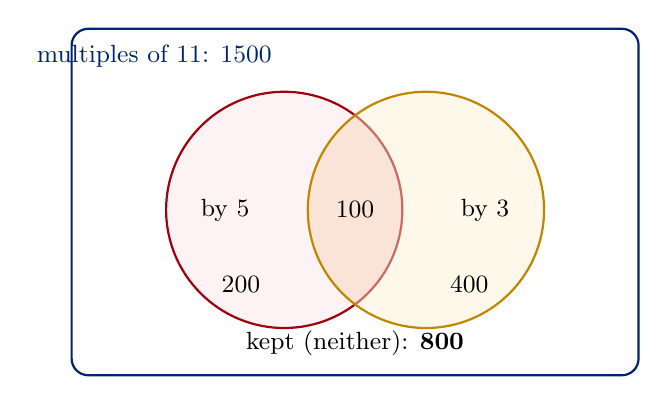
\begin{tikzpicture}[font=\small]
  \draw[rounded corners=6pt, thick, armBlue!70!black] (-3.6,-2.1) rectangle (3.6,2.3);
  \node[armBlue!70!black] at (-2.55,1.95) {multiples of $11$: $1500$};
  \begin{scope}
    \clip (-0.9,0) circle (1.5);
    \fill[armRed!18] (0.9,0) circle (1.5);
  \end{scope}
  \draw[armRed!75!black, thick, fill=armRed!10, fill opacity=0.45] (-0.9,0) circle (1.5);
  \draw[armOrange!80!black, thick, fill=armOrange!18, fill opacity=0.45] (0.9,0) circle (1.5);
  \node at (-1.65,0) {by $5$};
  \node at ( 1.65,0) {by $3$};
  \node at (-1.45,-0.95) {$200$};   % only by 5 (within 11): 300-100
  \node at ( 1.45,-0.95) {$400$};   % only by 3 (within 11): 500-100
  \node at ( 0,-0.0) {$100$};       % both
  \node at ( 0,-1.7) {kept (neither): $\mathbf{800}$};
\end{tikzpicture}
\end{center}

% ============================================================================
\section*{Problem 10 - Triangles in a side-8 subdivided triangle}

\begin{problembox}[10]
Each side of triangle $ABC$ is divided into $8$ equal parts, and through the division points all
lines parallel to the three sides are drawn, producing a triangular grid. Count all triangles whose
vertices are grid points (the corners $A,B,C$ count as grid points) and whose three sides are each
parallel to a side of $ABC$. This includes triangles in the same orientation as $ABC$
(\textbf{upward}) and the inverted ones (\textbf{downward}).
\end{problembox}

\begin{ideabox}
\textquotedbl{}Sides parallel to $ABC$\textquotedbl{} means every triangle we count is similar to
$ABC$ and sits squarely on the grid; there are only two possible orientations, \textbf{upward}
(pointing the same way as $ABC$) and \textbf{downward} (inverted). The grid has small upward unit
triangles and small downward unit triangles, and a bigger triangle of either orientation is just a
union of small ones. So the plan is: count upward triangles of every size, count downward triangles
of every size, and add.

Why split by orientation? Because the two families obey \emph{different} size limits. An upward
triangle of side $k$ fits as long as $k\le n$. But a downward triangle of side $k$ needs room on all
sides; it only fits when $k$ is at most $\lfloor n/2\rfloor$, which is why large inverted triangles
simply do not exist. Keeping the two counts separate is what makes the problem manageable. Here
$n=8$.
\end{ideabox}

\textbf{Step 1 - Upward triangles of side $k$.}
An upward triangle of side $k$ is fixed by the position of its top vertex. That vertex can sit
anywhere that still leaves room for the side-$k$ triangle below it, and those positions form a
triangular array of side $n-k$, which holds $1+2+\dots+(n-k+1)=\frac{(n-k+1)(n-k+2)}{2}$ points.
Each size count is itself a binomial, $\frac{(n-k+1)(n-k+2)}{2}=\binom{n-k+2}{2}$, so summing over
all sizes $k=1,\dots,8$ is $\binom{2}{2}+\binom{3}{2}+\dots+\binom{9}{2}$. By the hockey-stick
identity $\bigl(\sum_{m=2}^{n+1}\binom{m}{2}=\binom{n+2}{3}\bigr)$ this collapses to a single
binomial coefficient:
$$\sum_{k=1}^{8}\frac{(n-k+1)(n-k+2)}{2}=\binom{n+2}{3}=\binom{10}{3}=120.$$
Term by term: $36,28,21,15,10,6,3,1$ for $k=1,\dots,8$, and $36+28+21+15+10+6+3+1=120$.

\textbf{Step 2 - Downward (inverted) triangles of side $k$.}
A downward triangle of side $k$ exists only for $k\le\lfloor 8/2\rfloor=4$, and there are
$\frac{(n-2k+1)(n-2k+2)}{2}$ of side $k$:
$$k=1:\ \tfrac{7\cdot 8}{2}=28,\quad k=2:\ \tfrac{5\cdot 6}{2}=15,\quad
  k=3:\ \tfrac{3\cdot 4}{2}=6,\quad k=4:\ \tfrac{1\cdot 2}{2}=1.$$
Sum of downward triangles: $28+15+6+1=50$.

\textbf{Step 3 - Total.}
$$\underbrace{120}_{\text{upward}}+\underbrace{50}_{\text{downward}}=170.$$

\textbf{Always check.} A direct computer enumeration over the triangular grid (test every triple of
grid points forming an upward or a downward triangle of any size) returns $120$ upward and $50$
downward, total $170$. A known closed form for a side-$n$ triangle also agrees: for $n=8$,
$\big\lfloor \frac{n(n+2)(2n+1)}{8}\big\rfloor=\frac{8\cdot 10\cdot 17}{8}=170$. \checkmark

\answer{$120\ (\text{upward})+50\ (\text{downward})=170$}

\medskip
\textbf{Important reading note.} If the intended count were only triangles \emph{similarly oriented}
to $ABC$ (upward), the answer would be $120$. The statement asks for all grid triangles with sides
parallel to $ABC$, which includes the inverted ones, so the full total is $\mathbf{170}$. We report
the breakdown so either reading is covered.

\begin{methodbox}
\textbf{Transferable technique - count by size and by orientation.} In a triangular grid of side
$n$: upward triangles total $\binom{n+2}{3}$ (sum of $\frac{(n-k+1)(n-k+2)}{2}$). Downward triangles
of side $k$ exist only for $2k\le n$ and number $\frac{(n-2k+1)(n-2k+2)}{2}$. When a figure can
appear in more than one orientation, split the count by orientation first - the orientations usually
have different feasibility limits.
\end{methodbox}

\medskip
\textbf{The grid (here drawn at side $4$ for clarity).} Upward triangles point up like $ABC$;
the one shaded triangle is \emph{downward}. A downward triangle of side $k$ fits only when
$2k\le n$ (it must sit inside an upward triangle of side $2k$), which is why the big inverted ones
run out of room.

\begin{center}
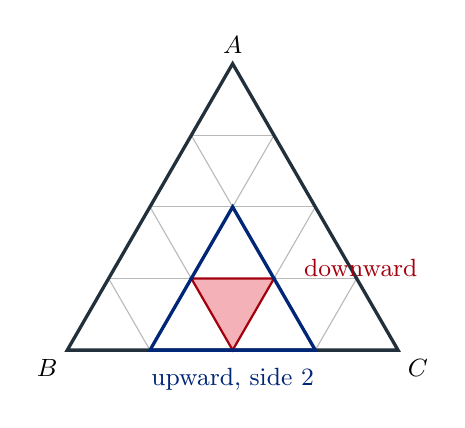
\begin{tikzpicture}[scale=1.05, font=\small]
  \def\nn{4}
  % grid points P(i,j) = i*(1,0) + j*(0.5, h)
  \pgfmathsetmacro{\hh}{sqrt(3)/2}
  % draw the three families of grid lines for n=4
  % lines parallel to base (horizontal), rows j=0..n
  \foreach \j in {0,...,4}{
    \pgfmathsetmacro{\xs}{\j*0.5}
    \pgfmathsetmacro{\ys}{\j*\hh}
    \pgfmathsetmacro{\xe}{(\nn-\j)+\j*0.5}
    \draw[gray!55] (\xs,\ys) -- (\xe,\ys);
  }
  % lines parallel to left side: from base going up-right
  \foreach \i in {0,...,4}{
    \pgfmathsetmacro{\xs}{\i}
    \pgfmathsetmacro{\xe}{\i+(\nn-\i)*0.5}
    \pgfmathsetmacro{\ye}{(\nn-\i)*\hh}
    \draw[gray!55] (\xs,0) -- (\xe,\ye);
  }
  % lines parallel to right side: from base going up-left
  \foreach \i in {0,...,4}{
    \pgfmathsetmacro{\xs}{\i}
    \pgfmathsetmacro{\xe}{\i*0.5}
    \pgfmathsetmacro{\ye}{\i*\hh}
    \draw[gray!55] (\xs,0) -- (\xe,\ye);
  }
  % outline ABC
  \draw[very thick, ink] (0,0) -- (4,0) -- (2,{4*\hh}) -- cycle;
  \node[below left] at (0,0) {$B$};
  \node[below right] at (4,0) {$C$};
  \node[above] at (2,{4*\hh}) {$A$};
  % a shaded downward unit triangle: vertices P(1,0),P(2,0) up-pointing? choose a downward one.
  % downward unit triangle with vertices P(1,1),P(2,0)? Let's pick:
  % downward unit: (i+1,j),(i,j+1),(i+1,j+1) for i=1,j=0 -> P(2,0),P(1,1),P(2,1)
  \pgfmathsetmacro{\hh}{sqrt(3)/2}
  \coordinate (d1) at (2,0);
  \coordinate (d2) at ({1+0.5},{\hh});
  \coordinate (d3) at ({2+0.5},{\hh});
  \fill[armRed!30] (d1) -- (d2) -- (d3) -- cycle;
  \draw[armRed!75!black, thick] (d1) -- (d2) -- (d3) -- cycle;
  \node[armRed!75!black] at (3.55,1.0) {downward};
  % an upward triangle of side 2 outlined in blue
  \draw[armBlue!75!black, very thick]
     (1,0) -- (3,0) -- (2,{2*\hh}) -- cycle;
  \node[armBlue!75!black] at (2,-0.35) {upward, side $2$};
\end{tikzpicture}
\end{center}

\textbf{Counts by size for $n=8$ (what we actually summed):}
\begin{center}
\small
\begin{tabular}{@{}c|cccccccc|c@{}}
\toprule
side $k$ & 1 & 2 & 3 & 4 & 5 & 6 & 7 & 8 & total\\
\midrule
upward   & 36 & 28 & 21 & 15 & 10 & 6 & 3 & 1 & \textbf{120}\\
downward & 28 & 15 & 6  & 1  & 0 & 0 & 0 & 0 & \textbf{50}\\
\bottomrule
\end{tabular}
\end{center}

% ============================================================================
\section*{Problem 12 - Bounded integer solutions of a linear equation}

\begin{problembox}[12]
Find the number of integer solutions of the system
$$x_1+x_2+x_3=40,\qquad 4\le x_1\le 15,\quad 9\le x_2\le 18,\quad 5\le x_3\le 16.$$
\end{problembox}

\begin{ideabox}
Two obstacles stand between us and a plain stars-and-bars count: the variables have \textbf{lower}
bounds (they do not start at $0$) and \textbf{upper} bounds (they cannot grow without limit). We
remove them one at a time.

\textbf{Lower bounds are free:} substitute $y_i=x_i-(\text{its minimum})$, so each $y_i\ge 0$ and the
total drops accordingly. \textbf{Upper bounds need inclusion-exclusion:} first count solutions
ignoring the upper caps (easy stars and bars), then subtract the \textquotedbl{}illegal\textquotedbl{}
solutions where some $y_i$ overshoots its cap. The clever part: \textquotedbl{}$y_i$ exceeds its cap
$c_i$\textquotedbl{} means \textquotedbl{}$y_i\ge c_i+1$\textquotedbl{}, which we enforce by handing
$c_i+1$ units to $y_i$ up front and counting the rest freely. Overshoots of two variables at once get
subtracted twice, so IEP adds them back. The whole solution is one tidy alternating sum.
\end{ideabox}

\textbf{Step 1 - Kill the lower bounds.}
Let $y_1=x_1-4,\ y_2=x_2-9,\ y_3=x_3-5$. Then $y_i\ge 0$ and
$$y_1+y_2+y_3=40-4-9-5=22,\qquad 0\le y_1\le 11,\ \ 0\le y_2\le 9,\ \ 0\le y_3\le 11.$$
(The caps are $15-4=11$, $18-9=9$, $16-5=11$.)

\textbf{Step 2 - Count ignoring the upper caps.}
Nonnegative solutions of $y_1+y_2+y_3=22$ by stars and bars:
$$\binom{22+3-1}{3-1}=\binom{24}{2}=276.$$

\textbf{Step 3 - Subtract single overshoots.}
\textquotedbl{}$y_i$ over its cap\textquotedbl{} means $y_i\ge \text{cap}+1$; give it that many units
and count solutions of the reduced total $22-(\text{cap}+1)$:
$$|y_1\ge 12|=\binom{(22-12)+2}{2}=\binom{12}{2}=66,\quad
  |y_2\ge 10|=\binom{(22-10)+2}{2}=\binom{14}{2}=91,$$
$$|y_3\ge 12|=\binom{(22-12)+2}{2}=\binom{12}{2}=66.$$

\textbf{Step 4 - Add back double overshoots.}
Two caps exceeded at once (give both their $\text{cap}+1$ units, then count the rest):
$$|y_1\ge12,\,y_2\ge10|=\binom{(22-12-10)+2}{2}=\binom{2}{2}=1,\quad
  |y_2\ge10,\,y_3\ge12|=\binom{2}{2}=1,$$
$$|y_1\ge12,\,y_3\ge12|:\ 22-12-12=-2<0\ \Rightarrow\ 0.$$
All three caps at once needs $12+10+12=34>22$ units, impossible, so the triple term is $0$.

\textbf{Step 5 - Assemble (inclusion-exclusion).}
$$276-(66+91+66)+(1+1+0)-0=276-223+2=55.$$

\textbf{Always check.} A brute-force triple loop over $x_1\in[4,15],\,x_2\in[9,18],\,x_3\in[5,16]$
counting those with $x_1+x_2+x_3=40$ returns exactly $55$. \checkmark

\answer{$\displaystyle \binom{24}{2}-\Big[\binom{12}{2}+\binom{14}{2}+\binom{12}{2}\Big]+\big[1+1\big]=55$}

\begin{methodbox}
\textbf{Transferable technique - bounded compositions.} To count integer solutions of
$x_1+\dots+x_k=N$ with $a_i\le x_i\le b_i$:
\begin{enumerate}[nosep,leftmargin=2em]
  \item Substitute $y_i=x_i-a_i$ to make all lower bounds $0$ (and lower $N$ by $\sum a_i$).
  \item Count without upper caps: $\binom{N'+k-1}{k-1}$.
  \item By IEP, subtract/add terms where a chosen subset $S$ of variables overshoots: each such
        variable contributes $(\text{cap}_i+1)$ removed from the total, with sign $(-1)^{|S|}$. Drop
        any term whose remaining total goes negative (it contributes $0$).
\end{enumerate}
\end{methodbox}

\medskip
\textbf{The IEP bookkeeping at a glance.}
\begin{center}
\small
\renewcommand{\arraystretch}{1.15}
\begin{tabular}{@{}llrcr@{}}
\toprule
overshoot set & remaining total & $\binom{\cdot+2}{2}$ & sign & contribution\\
\midrule
none                 & $22$ & $276$ & $+$ & $+276$\\
$y_1\ge12$           & $10$ & $66$  & $-$ & $-66$\\
$y_2\ge10$           & $12$ & $91$  & $-$ & $-91$\\
$y_3\ge12$           & $10$ & $66$  & $-$ & $-66$\\
$y_1\ge12,\,y_2\ge10$& $0$  & $1$   & $+$ & $+1$\\
$y_2\ge10,\,y_3\ge12$& $0$  & $1$   & $+$ & $+1$\\
$y_1\ge12,\,y_3\ge12$& $-2$ & $0$   & $+$ & $0$\\
all three            & $-12$& $0$   & $-$ & $0$\\
\midrule
\multicolumn{4}{r}{\textbf{net total (sum of contributions)}} & $\mathbf{55}$\\
\bottomrule
\end{tabular}
\end{center}

\end{document}
